\documentclass[twoside]{book}

% Packages required by doxygen
\usepackage{calc}
\usepackage{doxygen}
\usepackage{graphicx}
\usepackage[utf8]{inputenc}
\usepackage{makeidx}
\usepackage{multicol}
\usepackage{multirow}
\usepackage{textcomp}
\usepackage[table]{xcolor}

% Font selection
\usepackage[T1]{fontenc}
\usepackage{mathptmx}
\usepackage[scaled=.90]{helvet}
\usepackage{courier}
\usepackage{amssymb}
\usepackage{sectsty}
\renewcommand{\familydefault}{\sfdefault}
\allsectionsfont{%
  \fontseries{bc}\selectfont%
  \color{darkgray}%
}
\renewcommand{\DoxyLabelFont}{%
  \fontseries{bc}\selectfont%
  \color{darkgray}%
}

% Page & text layout
\usepackage{geometry}
\geometry{%
  a4paper,%
  top=2.5cm,%
  bottom=2.5cm,%
  left=2.5cm,%
  right=2.5cm%
}
\tolerance=750
\hfuzz=15pt
\hbadness=750
\setlength{\emergencystretch}{15pt}
\setlength{\parindent}{0cm}
\setlength{\parskip}{0.2cm}
\makeatletter
\renewcommand{\paragraph}{%
  \@startsection{paragraph}{4}{0ex}{-1.0ex}{1.0ex}{%
    \normalfont\normalsize\bfseries\SS@parafont%
  }%
}
\renewcommand{\subparagraph}{%
  \@startsection{subparagraph}{5}{0ex}{-1.0ex}{1.0ex}{%
    \normalfont\normalsize\bfseries\SS@subparafont%
  }%
}
\makeatother

% Headers & footers
\usepackage{fancyhdr}
\pagestyle{fancyplain}
\fancyhead[LE]{\fancyplain{}{\bfseries\thepage}}
\fancyhead[CE]{\fancyplain{}{}}
\fancyhead[RE]{\fancyplain{}{\bfseries\leftmark}}
\fancyhead[LO]{\fancyplain{}{\bfseries\rightmark}}
\fancyhead[CO]{\fancyplain{}{}}
\fancyhead[RO]{\fancyplain{}{\bfseries\thepage}}
\fancyfoot[LE]{\fancyplain{}{}}
\fancyfoot[CE]{\fancyplain{}{}}
\fancyfoot[RE]{\fancyplain{}{\bfseries\scriptsize Generated on Tue Feb 23 2021 09\-:34\-:15 for K\-V\-C\-G Fault Tolerance by Doxygen }}
\fancyfoot[LO]{\fancyplain{}{\bfseries\scriptsize Generated on Tue Feb 23 2021 09\-:34\-:15 for K\-V\-C\-G Fault Tolerance by Doxygen }}
\fancyfoot[CO]{\fancyplain{}{}}
\fancyfoot[RO]{\fancyplain{}{}}
\renewcommand{\footrulewidth}{0.4pt}
\renewcommand{\chaptermark}[1]{%
  \markboth{#1}{}%
}
\renewcommand{\sectionmark}[1]{%
  \markright{\thesection\ #1}%
}

% Indices & bibliography
\usepackage{natbib}
\usepackage[titles]{tocloft}
\setcounter{tocdepth}{3}
\setcounter{secnumdepth}{5}
\makeindex

% Hyperlinks (required, but should be loaded last)
\usepackage{ifpdf}
\ifpdf
  \usepackage[pdftex,pagebackref=true]{hyperref}
\else
  \usepackage[ps2pdf,pagebackref=true]{hyperref}
\fi
\hypersetup{%
  colorlinks=true,%
  linkcolor=blue,%
  citecolor=blue,%
  unicode%
}

% Custom commands
\newcommand{\clearemptydoublepage}{%
  \newpage{\pagestyle{empty}\cleardoublepage}%
}


%===== C O N T E N T S =====

\begin{document}

% Titlepage & ToC
\hypersetup{pageanchor=false}
\pagenumbering{roman}
\begin{titlepage}
\vspace*{7cm}
\begin{center}%
{\Large K\-V\-C\-G Fault Tolerance }\\
\vspace*{1cm}
{\large Generated by Doxygen 1.8.5}\\
\vspace*{0.5cm}
{\small Tue Feb 23 2021 09:34:15}\\
\end{center}
\end{titlepage}
\clearemptydoublepage
\tableofcontents
\clearemptydoublepage
\pagenumbering{arabic}
\hypersetup{pageanchor=true}

%--- Begin generated contents ---
\chapter{Hierarchical Index}
\section{Class Hierarchy}
This inheritance list is sorted roughly, but not completely, alphabetically\-:\begin{DoxyCompactList}
\item \contentsline{section}{Node}{\pageref{classNode}}{}
\begin{DoxyCompactList}
\item \contentsline{section}{Client}{\pageref{classClient}}{}
\item \contentsline{section}{Server}{\pageref{classServer}}{}
\end{DoxyCompactList}
\end{DoxyCompactList}

\chapter{Class Index}
\section{Class List}
Here are the classes, structs, unions and interfaces with brief descriptions\-:\begin{DoxyCompactList}
\item\contentsline{section}{\hyperlink{classClient}{Client} }{\pageref{classClient}}{}
\item\contentsline{section}{\hyperlink{classNode}{Node} }{\pageref{classNode}}{}
\item\contentsline{section}{\hyperlink{classServer}{Server} }{\pageref{classServer}}{}
\end{DoxyCompactList}

\chapter{File Index}
\section{File List}
Here is a list of all documented files with brief descriptions\-:\begin{DoxyCompactList}
\item\contentsline{section}{/root/cjdambro/grad-\/school/\-C\-S\-E498/gits/fault-\/tolerance/include/\hyperlink{fault__tolerance_8h}{fault\-\_\-tolerance.\-h} \\*Public A\-P\-I for K\-V\-C\-G Fault Tolerance protocol }{\pageref{fault__tolerance_8h}}{}
\end{DoxyCompactList}

\chapter{Class Documentation}
\hypertarget{classClient}{\section{Client Class Reference}
\label{classClient}\index{Client@{Client}}
}
Inheritance diagram for Client\-:\begin{figure}[H]
\begin{center}
\leavevmode
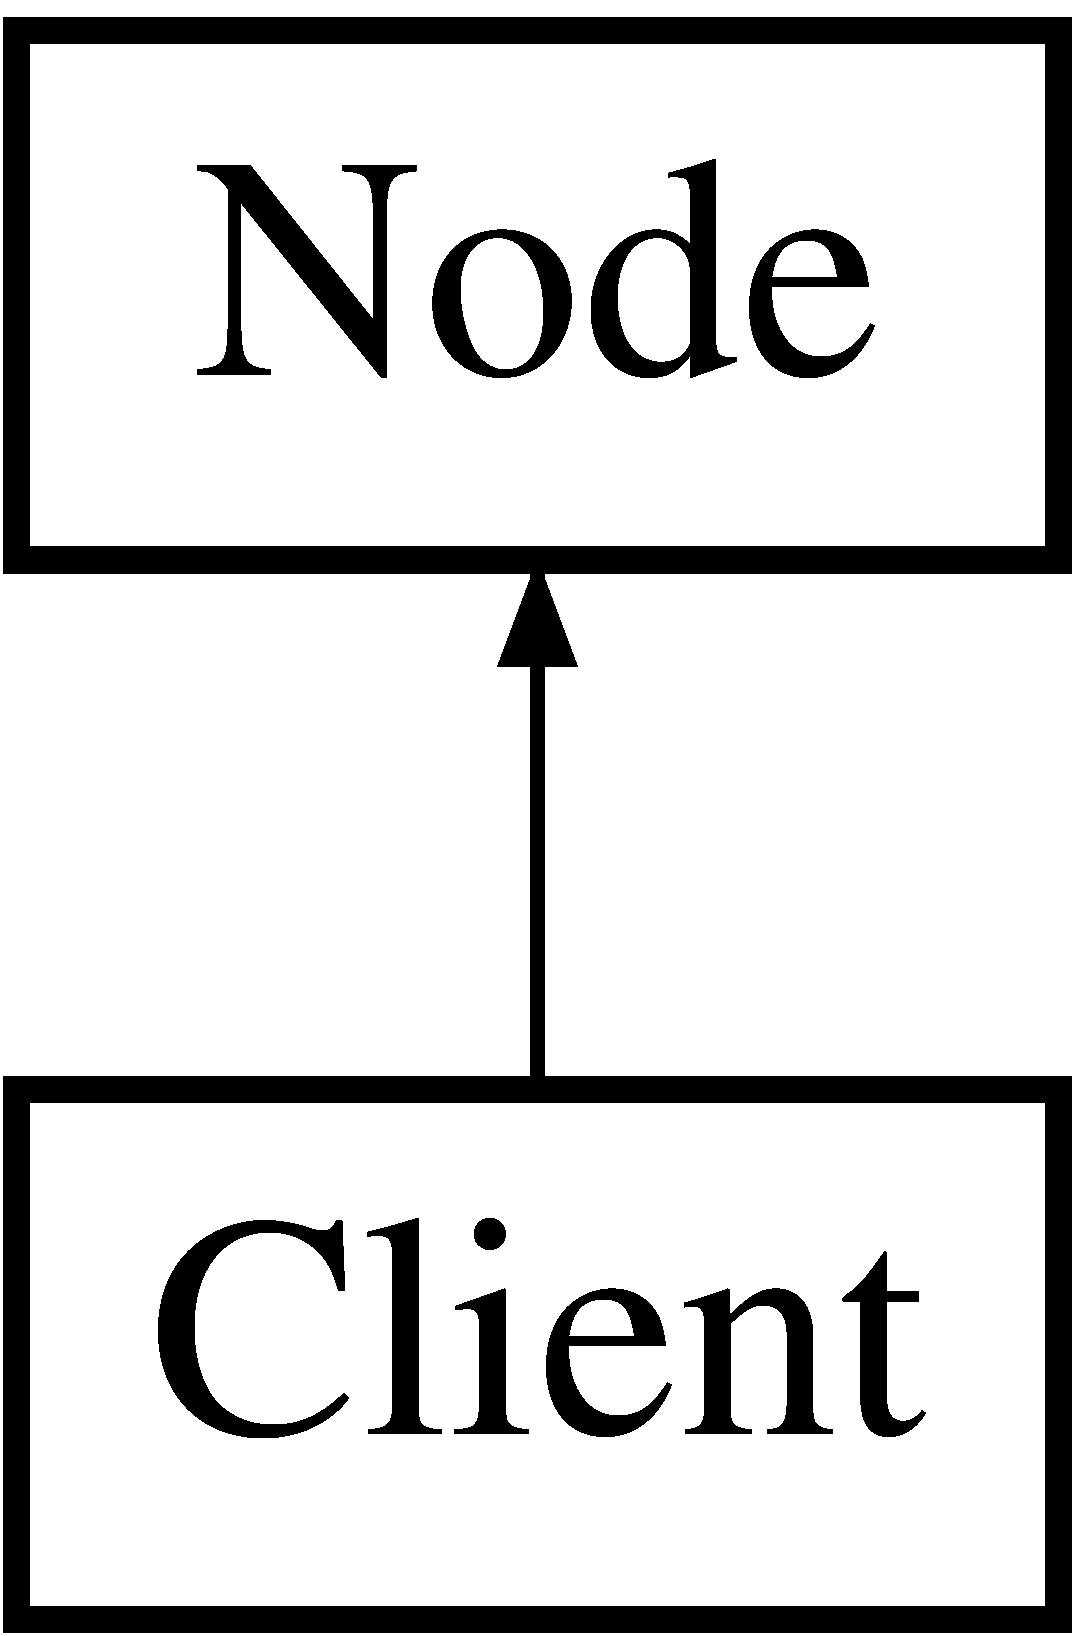
\includegraphics[height=2.000000cm]{classClient}
\end{center}
\end{figure}
\subsection*{Public Member Functions}
\begin{DoxyCompactItemize}
\item 
int \hyperlink{classClient_a5de857af6e3c568925ecd342314617d7}{initialize} ()
\end{DoxyCompactItemize}
\subsection*{Additional Inherited Members}


\subsection{Member Function Documentation}
\hypertarget{classClient_a5de857af6e3c568925ecd342314617d7}{\index{Client@{Client}!initialize@{initialize}}
\index{initialize@{initialize}!Client@{Client}}
\subsubsection[{initialize}]{\setlength{\rightskip}{0pt plus 5cm}int Client\-::initialize (
\begin{DoxyParamCaption}
{}
\end{DoxyParamCaption}
)\hspace{0.3cm}{\ttfamily [virtual]}}}\label{classClient_a5de857af6e3c568925ecd342314617d7}
Initialize client


\begin{DoxyParams}{Parameters}
{\em None} & \\
\hline
\end{DoxyParams}
\begin{DoxyReturn}{Returns}
integer 
\end{DoxyReturn}


Reimplemented from \hyperlink{classNode}{Node}.



The documentation for this class was generated from the following file\-:\begin{DoxyCompactItemize}
\item 
/root/cjdambro/grad-\/school/\-C\-S\-E498/gits/fault-\/tolerance/include/\hyperlink{fault__tolerance_8h}{fault\-\_\-tolerance.\-h}\end{DoxyCompactItemize}

\hypertarget{classNode}{\section{Node Class Reference}
\label{classNode}\index{Node@{Node}}
}
Inheritance diagram for Node\-:\begin{figure}[H]
\begin{center}
\leavevmode
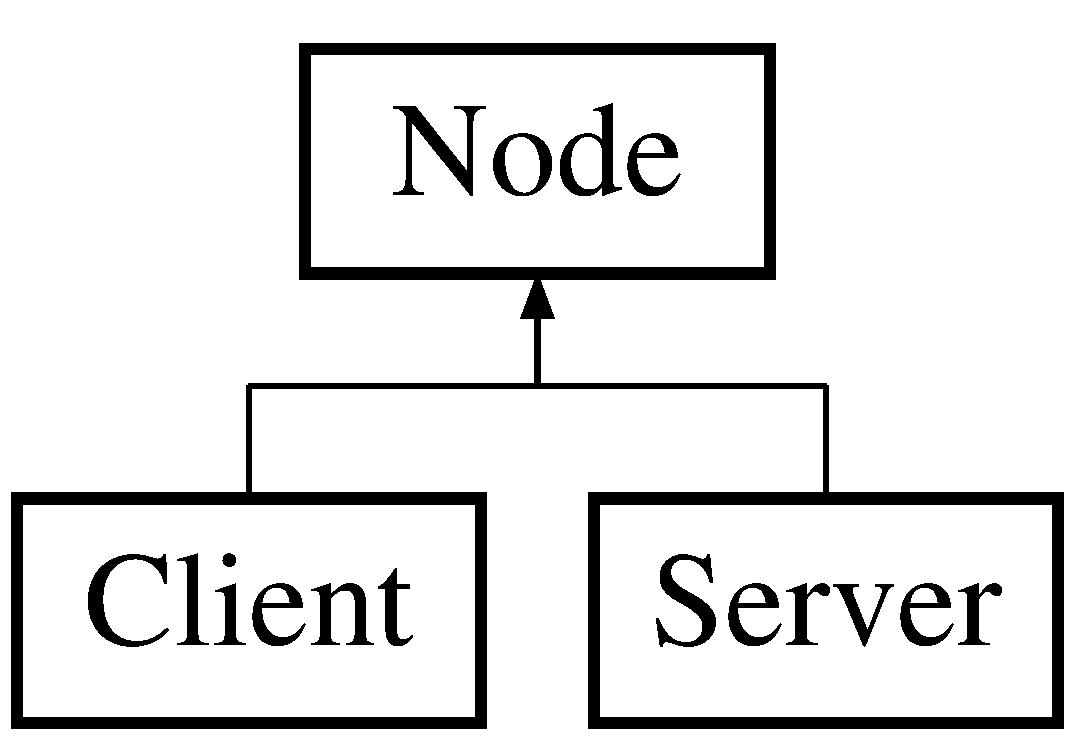
\includegraphics[height=2.000000cm]{classNode}
\end{center}
\end{figure}
\subsection*{Public Member Functions}
\begin{DoxyCompactItemize}
\item 
\hypertarget{classNode_acfbc12d3b7d414fb12811041b04a1809}{virtual int {\bfseries initialize} ()}\label{classNode_acfbc12d3b7d414fb12811041b04a1809}

\item 
\hypertarget{classNode_af79916b6bb2580b7cf9397bdeb172988}{void {\bfseries set\-Name} (std\-::string n)}\label{classNode_af79916b6bb2580b7cf9397bdeb172988}

\item 
\hypertarget{classNode_a3e5ac6b5881a3a9d82f3112953c1e546}{std\-::string {\bfseries get\-Name} ()}\label{classNode_a3e5ac6b5881a3a9d82f3112953c1e546}

\end{DoxyCompactItemize}
\subsection*{Protected Attributes}
\begin{DoxyCompactItemize}
\item 
\hypertarget{classNode_a9f5a57e15567a0b92cb8d25bcec7bd24}{std\-::string {\bfseries hostname}}\label{classNode_a9f5a57e15567a0b92cb8d25bcec7bd24}

\end{DoxyCompactItemize}


The documentation for this class was generated from the following file\-:\begin{DoxyCompactItemize}
\item 
/root/cjdambro/grad-\/school/\-C\-S\-E498/gits/fault-\/tolerance/include/\hyperlink{fault__tolerance_8h}{fault\-\_\-tolerance.\-h}\end{DoxyCompactItemize}

\hypertarget{classServer}{\section{Server Class Reference}
\label{classServer}\index{Server@{Server}}
}
Inheritance diagram for Server\-:\begin{figure}[H]
\begin{center}
\leavevmode
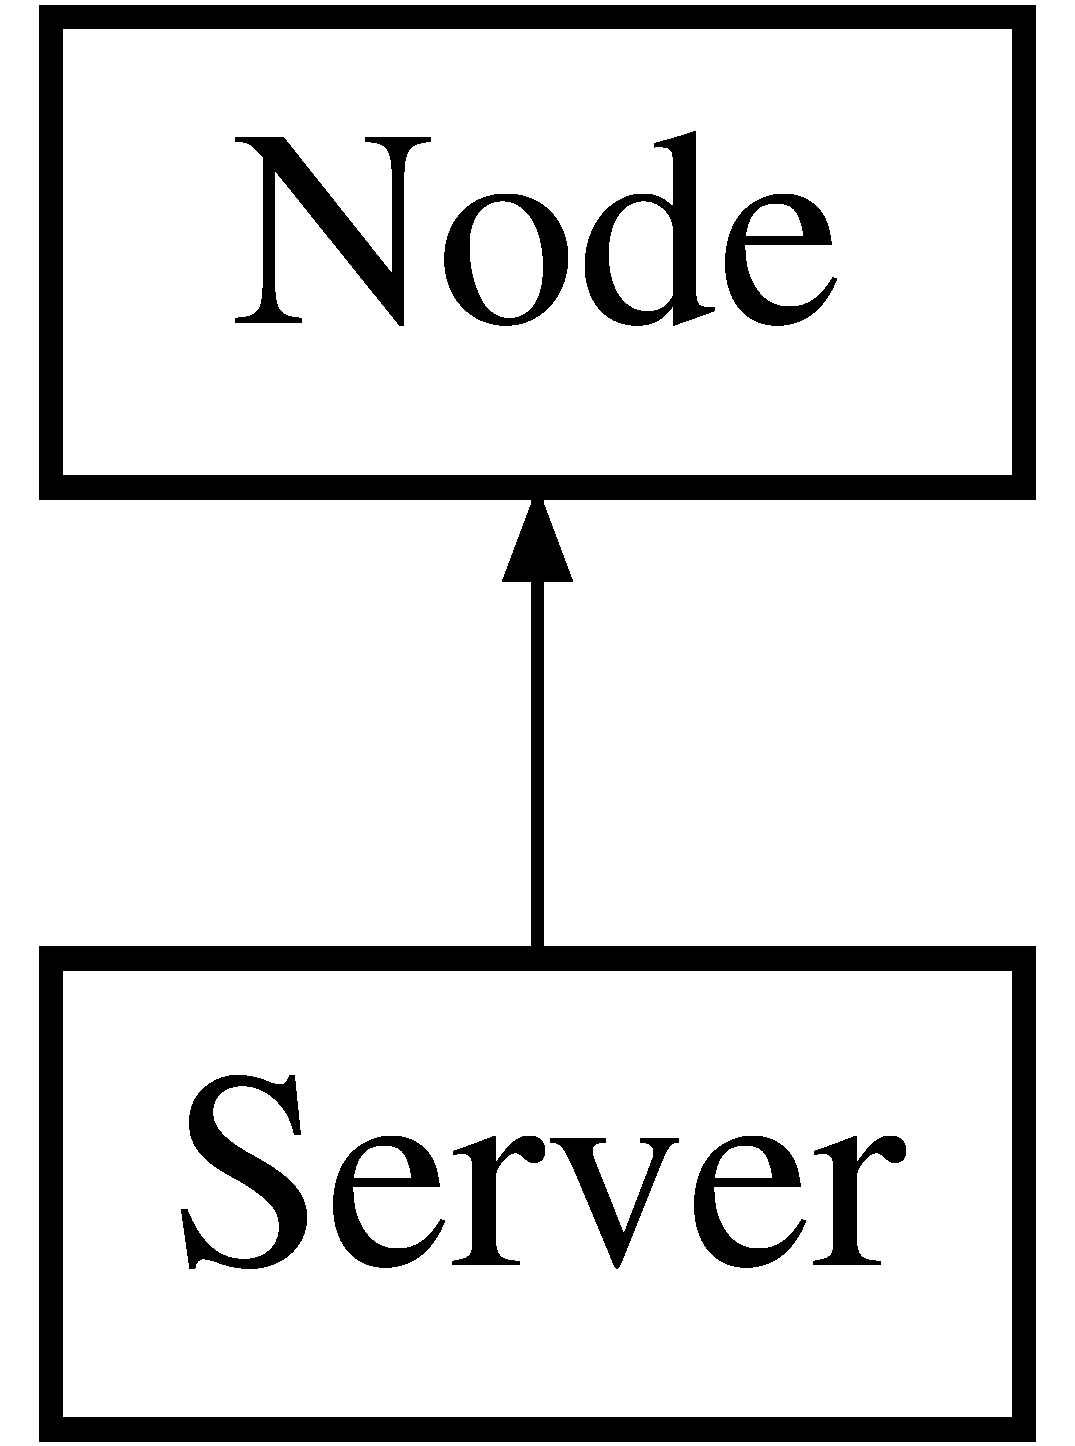
\includegraphics[height=2.000000cm]{classServer}
\end{center}
\end{figure}
\subsection*{Public Member Functions}
\begin{DoxyCompactItemize}
\item 
int \hyperlink{classServer_ae94d08657f48a3b51b411463f1137375}{initialize} ()
\item 
std\-::vector$<$ std\-::pair$<$ int, \\*
int $>$ $>$ \hyperlink{classServer_ad303d839086eee11137e6fc4a4bb95ab}{get\-Primary\-Keys} ()
\item 
bool \hyperlink{classServer_a395d7cb7194064c961710663926e4a3d}{add\-Key\-Range} (std\-::pair$<$ int, int $>$ key\-Range)
\item 
bool \hyperlink{classServer_a2f865f52beecb3be03eda85b4dc64e3e}{add\-Primary\-Server} (\hyperlink{classServer}{Server} $\ast$s)
\item 
bool \hyperlink{classServer_ab272570a3b1d8eb7f9037c9e7b4e5f2a}{add\-Backup\-Server} (\hyperlink{classServer}{Server} $\ast$s)
\item 
bool \hyperlink{classServer_a9bd7a3b2b12f2f5bddd68eb245111d02}{is\-Primary} (int key)
\end{DoxyCompactItemize}
\subsection*{Additional Inherited Members}


\subsection{Member Function Documentation}
\hypertarget{classServer_ab272570a3b1d8eb7f9037c9e7b4e5f2a}{\index{Server@{Server}!add\-Backup\-Server@{add\-Backup\-Server}}
\index{add\-Backup\-Server@{add\-Backup\-Server}!Server@{Server}}
\subsubsection[{add\-Backup\-Server}]{\setlength{\rightskip}{0pt plus 5cm}bool Server\-::add\-Backup\-Server (
\begin{DoxyParamCaption}
\item[{{\bf Server} $\ast$}]{s}
\end{DoxyParamCaption}
)}}\label{classServer_ab272570a3b1d8eb7f9037c9e7b4e5f2a}
Add server who is backing this one up


\begin{DoxyParams}{Parameters}
{\em s} & -\/ \hyperlink{classServer}{Server} to add to backup server list\\
\hline
\end{DoxyParams}
\begin{DoxyReturn}{Returns}
bool -\/ true if added successfully, false otherwise 
\end{DoxyReturn}
\hypertarget{classServer_a395d7cb7194064c961710663926e4a3d}{\index{Server@{Server}!add\-Key\-Range@{add\-Key\-Range}}
\index{add\-Key\-Range@{add\-Key\-Range}!Server@{Server}}
\subsubsection[{add\-Key\-Range}]{\setlength{\rightskip}{0pt plus 5cm}bool Server\-::add\-Key\-Range (
\begin{DoxyParamCaption}
\item[{std\-::pair$<$ int, int $>$}]{key\-Range}
\end{DoxyParamCaption}
)}}\label{classServer_a395d7cb7194064c961710663926e4a3d}
Add key range to primary list


\begin{DoxyParams}{Parameters}
{\em key\-Range} & -\/ std\-::pair$<$int, int$>$ of min and max key\\
\hline
\end{DoxyParams}
\begin{DoxyReturn}{Returns}
bool -\/ true if added successfully, false otherwise 
\end{DoxyReturn}
\hypertarget{classServer_a2f865f52beecb3be03eda85b4dc64e3e}{\index{Server@{Server}!add\-Primary\-Server@{add\-Primary\-Server}}
\index{add\-Primary\-Server@{add\-Primary\-Server}!Server@{Server}}
\subsubsection[{add\-Primary\-Server}]{\setlength{\rightskip}{0pt plus 5cm}bool Server\-::add\-Primary\-Server (
\begin{DoxyParamCaption}
\item[{{\bf Server} $\ast$}]{s}
\end{DoxyParamCaption}
)}}\label{classServer_a2f865f52beecb3be03eda85b4dc64e3e}
Add server who this one is backing up


\begin{DoxyParams}{Parameters}
{\em s} & -\/ \hyperlink{classServer}{Server} to add to primary server list\\
\hline
\end{DoxyParams}
\begin{DoxyReturn}{Returns}
bool -\/ true if added successfully, false otherwise 
\end{DoxyReturn}
\hypertarget{classServer_ad303d839086eee11137e6fc4a4bb95ab}{\index{Server@{Server}!get\-Primary\-Keys@{get\-Primary\-Keys}}
\index{get\-Primary\-Keys@{get\-Primary\-Keys}!Server@{Server}}
\subsubsection[{get\-Primary\-Keys}]{\setlength{\rightskip}{0pt plus 5cm}std\-::vector$<$std\-::pair$<$int, int$>$ $>$ Server\-::get\-Primary\-Keys (
\begin{DoxyParamCaption}
{}
\end{DoxyParamCaption}
)\hspace{0.3cm}{\ttfamily [inline]}}}\label{classServer_ad303d839086eee11137e6fc4a4bb95ab}
Get vector of primary key ranges


\begin{DoxyParams}{Parameters}
{\em None} & \\
\hline
\end{DoxyParams}
\begin{DoxyReturn}{Returns}
vector of min/max key range pairs 
\end{DoxyReturn}
\hypertarget{classServer_ae94d08657f48a3b51b411463f1137375}{\index{Server@{Server}!initialize@{initialize}}
\index{initialize@{initialize}!Server@{Server}}
\subsubsection[{initialize}]{\setlength{\rightskip}{0pt plus 5cm}int Server\-::initialize (
\begin{DoxyParamCaption}
{}
\end{DoxyParamCaption}
)\hspace{0.3cm}{\ttfamily [virtual]}}}\label{classServer_ae94d08657f48a3b51b411463f1137375}
Initialize server


\begin{DoxyParams}{Parameters}
{\em None} & \\
\hline
\end{DoxyParams}
\begin{DoxyReturn}{Returns}
integer 
\end{DoxyReturn}


Reimplemented from \hyperlink{classNode}{Node}.

\hypertarget{classServer_a9bd7a3b2b12f2f5bddd68eb245111d02}{\index{Server@{Server}!is\-Primary@{is\-Primary}}
\index{is\-Primary@{is\-Primary}!Server@{Server}}
\subsubsection[{is\-Primary}]{\setlength{\rightskip}{0pt plus 5cm}bool Server\-::is\-Primary (
\begin{DoxyParamCaption}
\item[{int}]{key}
\end{DoxyParamCaption}
)}}\label{classServer_a9bd7a3b2b12f2f5bddd68eb245111d02}
Check if server is running as primary for a given key


\begin{DoxyParams}{Parameters}
{\em None} & \\
\hline
\end{DoxyParams}
\begin{DoxyReturn}{Returns}
bool -\/ true if primary, false otherwise 
\end{DoxyReturn}


The documentation for this class was generated from the following file\-:\begin{DoxyCompactItemize}
\item 
/root/cjdambro/grad-\/school/\-C\-S\-E498/gits/fault-\/tolerance/include/\hyperlink{fault__tolerance_8h}{fault\-\_\-tolerance.\-h}\end{DoxyCompactItemize}

\chapter{File Documentation}
\hypertarget{fault__tolerance_8h}{\section{/root/cjdambro/grad-\/school/\-C\-S\-E498/gits/fault-\/tolerance/include/fault\-\_\-tolerance.h File Reference}
\label{fault__tolerance_8h}\index{/root/cjdambro/grad-\/school/\-C\-S\-E498/gits/fault-\/tolerance/include/fault\-\_\-tolerance.\-h@{/root/cjdambro/grad-\/school/\-C\-S\-E498/gits/fault-\/tolerance/include/fault\-\_\-tolerance.\-h}}
}


Public A\-P\-I for K\-V\-C\-G Fault Tolerance protocol.  


{\ttfamily \#include $<$string$>$}\\*
{\ttfamily \#include $<$vector$>$}\\*
{\ttfamily \#include \char`\"{}kvcg\-\_\-logging.\-h\char`\"{}}\\*
\subsection*{Classes}
\begin{DoxyCompactItemize}
\item 
class \hyperlink{classNode}{Node}
\item 
class \hyperlink{classServer}{Server}
\item 
class \hyperlink{classClient}{Client}
\end{DoxyCompactItemize}
\subsection*{Variables}
\begin{DoxyCompactItemize}
\item 
\hypertarget{fault__tolerance_8h_a87365e85ba252f204b46586cf378fd41}{std\-::string {\bfseries C\-F\-G\-\_\-\-F\-I\-L\-E}}\label{fault__tolerance_8h_a87365e85ba252f204b46586cf378fd41}

\end{DoxyCompactItemize}


\subsection{Detailed Description}
Public A\-P\-I for K\-V\-C\-G Fault Tolerance protocol. 
%--- End generated contents ---

% Index
\newpage
\phantomsection
\addcontentsline{toc}{part}{Index}
\printindex

\end{document}
